\documentclass{beamer}
\usetheme{Warsaw}
\usepackage{graphicx}
\useoutertheme{miniframes}

% Datos
\title{Event Driven Molecular Dynamics}
\author{Grupo 5}
\institute{ITBA}
\date{} % sin fecha
\setbeamertemplate{headline}[miniframes theme]
% Numerar diapositivas
\setbeamertemplate{footline}[frame number]

\begin{document}

% Portada
\begin{frame}
  \titlepage
\end{frame}

% Introducción
\section{Introducción}
\subsection{Sistema Real}
\begin{frame}{Gas ideal, sistema de partículas rígidas por eventos}
  \textbf{Trayectoria recta, colisiones elásticas y sin gravedad}
  \vspace{0.5cm}
  \begin{itemize}
    % Descripción del sistema real.
    \item N particulas en movimiento.
    \item Cada particula con su movimiento, posicion, radio y masa.
    \item Viajan sin fuerzas externas.
    \item Colisiones elásticas entre partículas.
    \item Simulacion de un sistema de eventos.
  \end{itemize}
  % imagen del sistema de eventos
  \begin{center}
    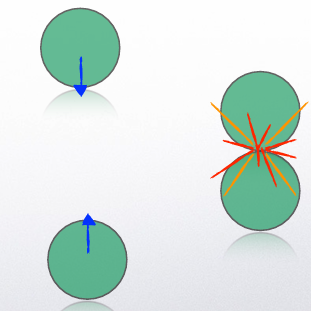
\includegraphics[width=0.3\linewidth]{photoMaterial/eventos_sistema_real.png}
  \end{center}
\end{frame}

\subsection{Modelo Matemático}
\begin{frame}{Modelo Matemático}
  \begin{itemize}
    \item Vuelo libre de las N particulas en un espacio 2D:
    \begin{itemize}
      \item $x_i(t) = x_i(0) + v_{x_i} t$
      \item $y_i(t) = y_i(0) + v_{y_i} t$
    \end{itemize}
    \item Calculo de tiempo de colision contra paredes:
    \begin{itemize}
      \item $t_{c} = \infty$ si $dv \cdot dr \geqslant 0$,
      \item $t_{c} = \infty$ si $d < 0$, siendo: $d = (dv \cdot dr)^2 - (dv \cdot dv)\cdot(dr \cdot dr - \sigma^2 )$,
      \item $\sigma = r_i + r_j$
      \item Colision con paredes espejan la velocidad en la normal de colision.
    \end{itemize}
  \end{itemize}
\end{frame}

% Colisiones entre particulas, formulas
\begin{frame}{Modelo Matemático}
  \begin{itemize}
    \item Calculo de impulso y velocidades post-colision de particulas:
      \begin{itemize}
        \item $J_x = J*dx/\sigma$
        \item $J_y = J*dy/\sigma$
        \item $J = \dfrac{2 m_i m_j}{m_i + m_j} \cdot \dfrac{dv \cdot dr}{\sigma}$
        \item $vx_i^d = vx_i^a + J_x/m_i$
        \item $vy_i^d = vy_i^a + J_y/m_i$
        \item $vx_j^d = vx_j^a - J_x/m_j$
        \item $vy_j^d = vy_j^a - J_y/m_j$
      \end{itemize}
    \item Coeficiente cuadratico medio: $<z^2> = 2Dt$
  \end{itemize}
\end{frame}

% Implementación
\section{Implementación}
\begin{frame}{Implementación}
  \begin{itemize}
    \item Arquitectura del código.
    \item Pseudocódigo o UML.
  \end{itemize}
  \begin{column}{0.5\textwidth}
    \begin{itemize}
      \item N particulas de radio $r_i$ y masa $m_i$.
      \item Posicion $(x_i, y_i)$ y velocidad $(v_{x_i}, v_{y_i})$.
      \item Colisiones elásticas entre partículas y paredes.
      \item Condiciones de frontera: Paredes rígidas.
    \end{itemize}
  \end{column}
\end{frame}
\begin{frame}{Implementación de vértices}
  % Consultar martina
  \begin{itemize}
    \item Arquitectura del código.
    \item Pseudocódigo o UML.
  \end{itemize}
  \begin{column}{0.5\textwidth}
    \begin{itemize}
      \item N particulas de radio $r_i$ y masa $m_i$.
      \item Posicion $(x_i, y_i)$ y velocidad $(v_{x_i}, v_{y_i})$.
      \item Colisiones elásticas entre partículas y paredes.
      \item Condiciones de frontera: Paredes rígidas.
    \end{itemize}
  \end{column}
\end{frame}

% Simulaciones

\begin{frame}{Geometría del sistema y ubicaciones iniciales}
  \small Dos cajas A y B, conectadas por una abertura de tamaño L.

  \vspace{0.5cm}
  \begin{center}
    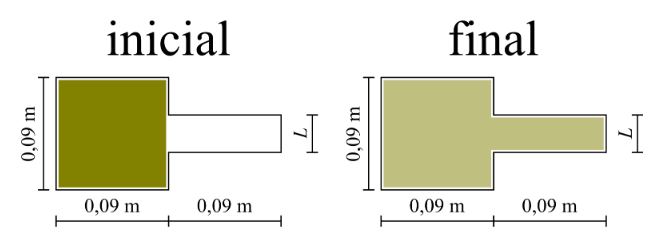
\includegraphics[width=0.5\linewidth]{photoMaterial/geometria.jpg}
  \end{center}
  \vspace{0.5cm}

  \small Las partículas se distribuyen uniformemente en la caja A al inicio de la simulación sin superponerse.
\end{frame}

\section{Simulaciones}
\subsection{Parámetros y observables}
\begin{frame}{Parámetros de la simulación}
  \textbf{Constantes}
    \begin{itemize}
      \item Numero de partículas: 250.
      \item Dimensiones caja A: \textit{0.09} m ancho x \textit{0.09} m alto.
      \item Dimensiones caja B: \textit{0.09} m ancho.
      \item Radio partículas: \textit{0.0015} m.
      \item Masa partículas: \textit{0.01} kg.
      \item Velocidad inicial: \textit{0.01} m/s.
      \item EPS: \textit{1e-12}.
    \end{itemize}
    \vspace{0.5cm}
    \textbf{Variables}
    \begin{itemize}
      \item L puede tomar los valores de: \textit{0.09} m, \textit{0.07} m, \textit{0.05} m y \textit{0.03} kg.
    \end{itemize}
  \end{frame}

\begin{frame}{Definición matemática de observables}
  \textbf{Observables}
  \begin{itemize}
    \item Presión en las cajas A y B.
    \item Calculándolas como la suma de los impúlsos por colisiones contra la pared por unidad de tiempo.
    \item Se obtiene con la fórmula:
      \begin{equation}
        P = \frac{1}{A} \sum J_i
      \end{equation}
  \end{itemize}
\end{frame}

% Resultados
\section{Resultados}
\subsection{Animaciones}
\begin{frame}{Animaciones}
  % Aquí va la imagen de un frame representativo
  \includegraphics[width=0.7\linewidth]{ejemplo.png}
  \vspace{0.3cm}
  \footnotesize Link al video: \url{https://youtube.com/...}
\end{frame}

\begin{frame}{Evolución temporal del observable}
  \begin{columns}
    \begin{column}{0.5\textwidth}
      \tiny \textit{Presión en función del tiempo para $L = 0.09$ m.}
      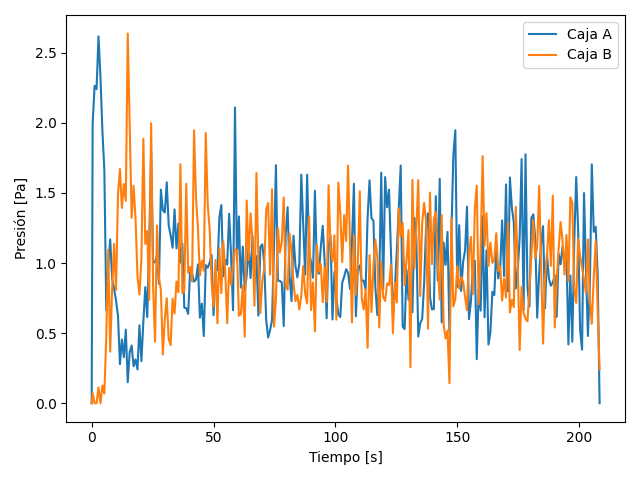
\includegraphics[width=\linewidth]{photoMaterial/pvt_09.png}
    \end{column}
    \begin{column}{0.5\textwidth}
      \tiny \textit{Presión en función del tiempo para $L = 0.07$ m.}
      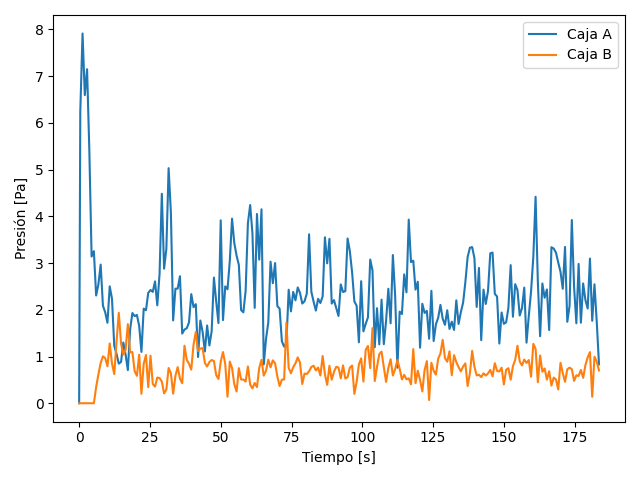
\includegraphics[width=\linewidth]{photoMaterial/pvt_07.png}
    \end{column}
    \end{columns}
    \tiny Podemos tomar estacionario a partir de los 20 segundos.
    \tiny Con: N = \textit{250}, r = \textit{0.0015} m, m = \textit{0.01} kg.
\end{frame}
\subsection{Primer estudio: Presión vs $A^{-1}$}
\begin{frame}{Evolución temporal del observable}
  \begin{columns}
    \begin{column}{0.5\textwidth}
      \scriptsize \textit{Presión en función del tiempo para $L = 0.05$ m.}
      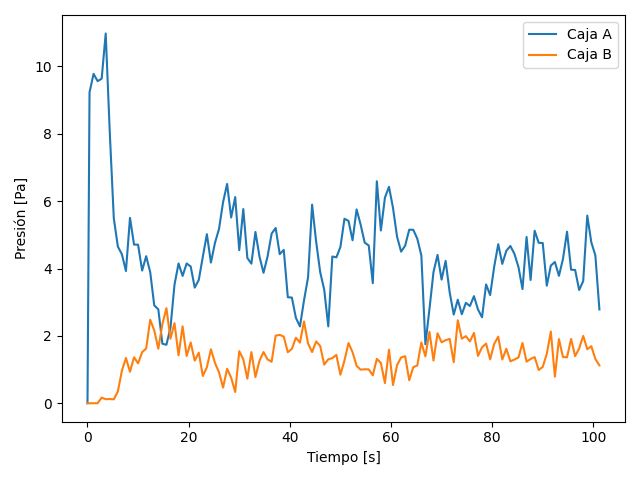
\includegraphics[width=\linewidth]{photoMaterial/pvt_05.png}
    \end{column}
    \begin{column}{0.5\textwidth}
      \scriptsize \textit{Presión en función del tiempo para $L = 0.03$ m.}
      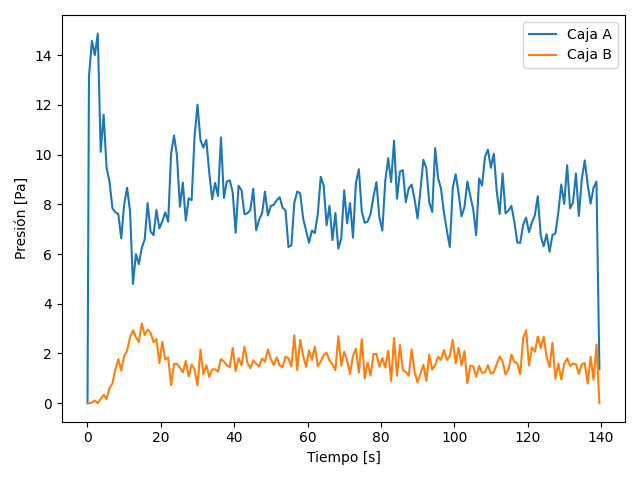
\includegraphics[width=\linewidth]{photoMaterial/pvt_03.png}
    \end{column}
  \end{columns}
  \tiny Podemos tomar estacionario a partir de los 20 segundos.
  \tiny Con: N = \textit{250}, r = \textit{0.0015} m, m = \textit{0.01} kg.
\end{frame}

\begin{frame}{Input vs Observable}
  \begin{columns}
    \begin{column}{0.40\textwidth}
      \scriptsize \text{Input}
      \begin{itemize}
        \item L = \textit{0.09} m, \textit{0.007} m, \textit{0.05} m, \textit{0.03} m. 
        \item Velocidad inicial = \textit{0.01} m/s.
        \item Radio partículas = \textit{0.0015} m.
        \item Masa partículas = \textit{0.01} kg.
        \item Número de partículas = 250.
      \end{itemize}
    \end{column}
    \begin{column}{0.60\textwidth}
      %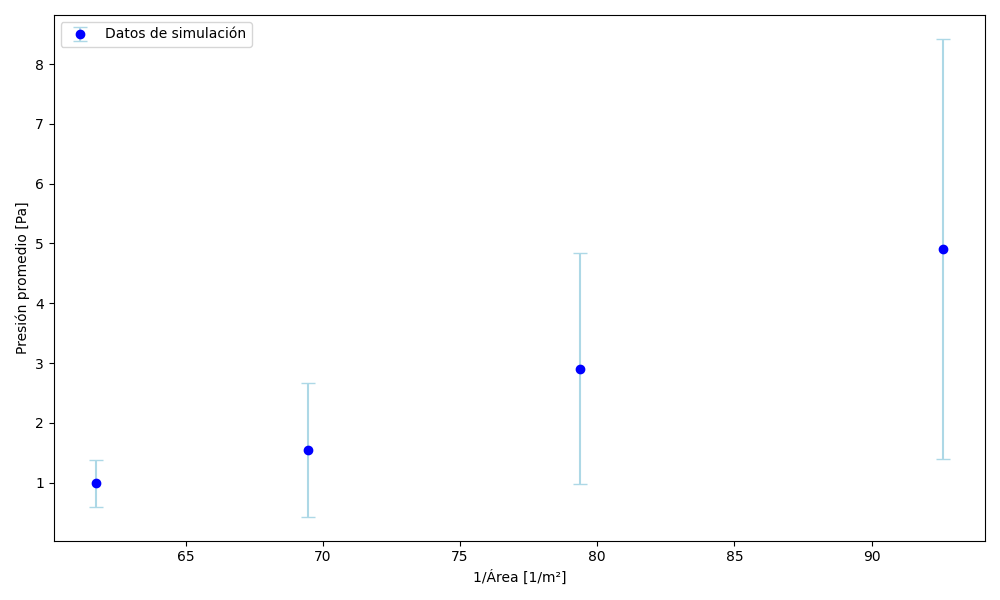
\includegraphics[width=0.75\linewidth]{photoMaterial/Presion_vs_area.png} ver si meterlo o no
      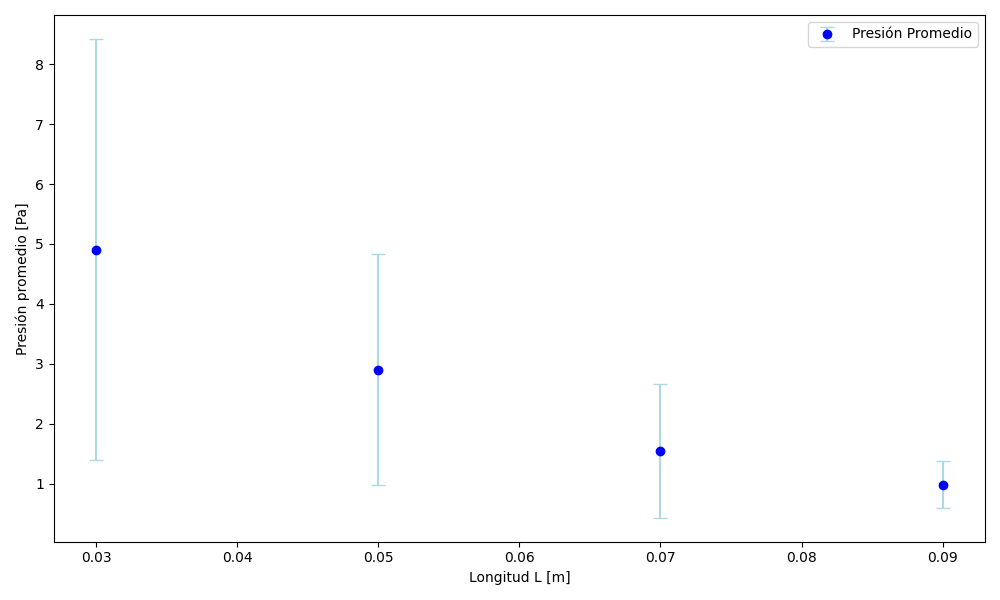
\includegraphics[width=1\linewidth]{photoMaterial/Presion_vs_L.png}
    \end{column}
  \end{columns}
\end{frame}

\begin{frame}{Input vs Observable}
  \begin{columns}
    \begin{column}{0.40\textwidth}
      \scriptsize \text{Input}
      \begin{itemize}
        \item L = \textit{0.09} m, \textit{0.007} m, \textit{0.05} m, \textit{0.03} m. 
        \item Velocidad inicial = \textit{0.01} m/s.
        \item Radio partículas = \textit{0.0015} m.
        \item Masa partículas = \textit{0.01} kg.
        \item Número de partículas = 250.
      \end{itemize}
    \end{column}
    \begin{column}{0.60\textwidth}
      %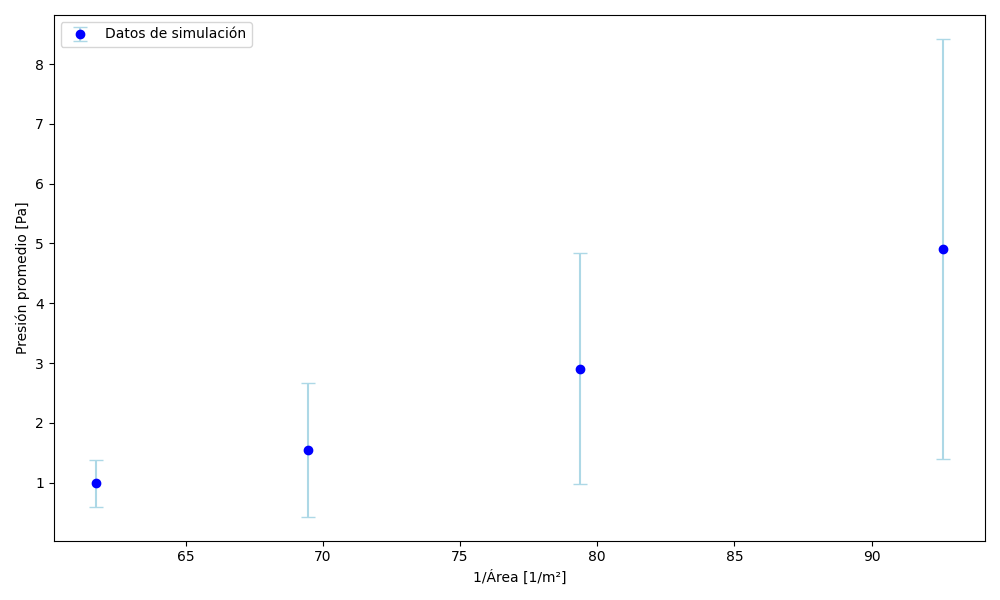
\includegraphics[width=0.75\linewidth]{photoMaterial/Presion_vs_area.png} ver si meterlo o no
      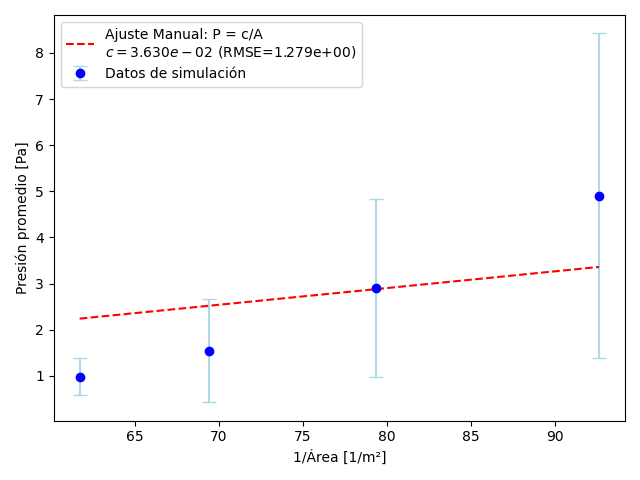
\includegraphics[width=1\linewidth]{photoMaterial/Presion_vs_area_ajuste.png}
    \end{column}
  \end{columns}
\end{frame}

\subsection{Segundo estudio: Coeficiente de difusión}
\begin{frame}{Coeficiente de difusión}
  \begin{columns}
    \begin{column}{0.30\textwidth}
      \scriptsize \text{Input}
      \begin{itemize}
        \item L = \textit{0.09} m. 
        \item Velocidad inicial = \textit{0.01} m/s.
        \item Radio partículas = \textit{0.0015} m.
        \item Masa partículas = \textit{0.01} kg.
        \item Número de partículas = 250.
      \end{itemize}
    \end{column}
    \begin{column}{0.70\textwidth}
      %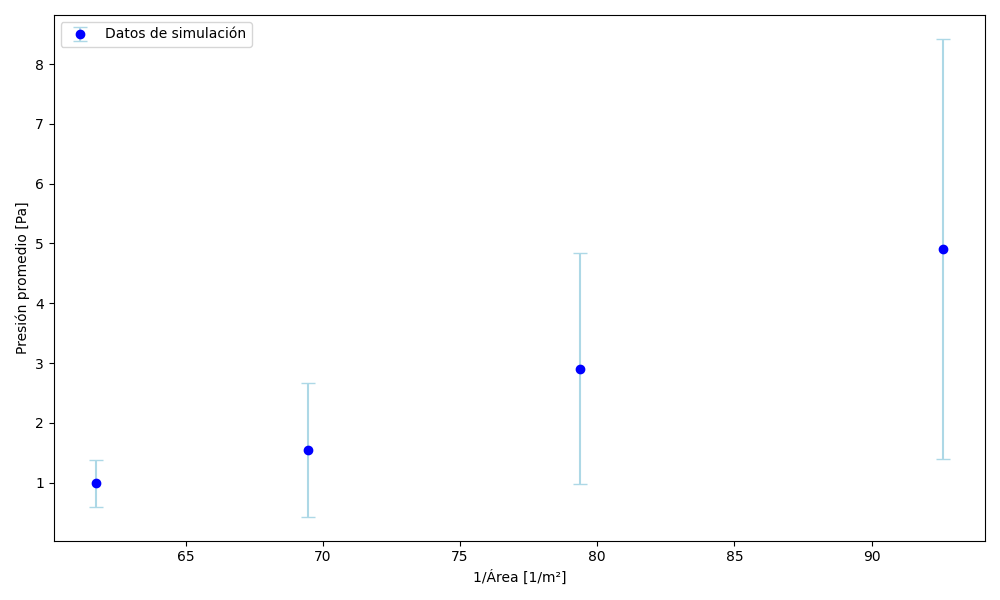
\includegraphics[width=0.75\linewidth]{photoMaterial/Presion_vs_area.png} ver si meterlo o no
      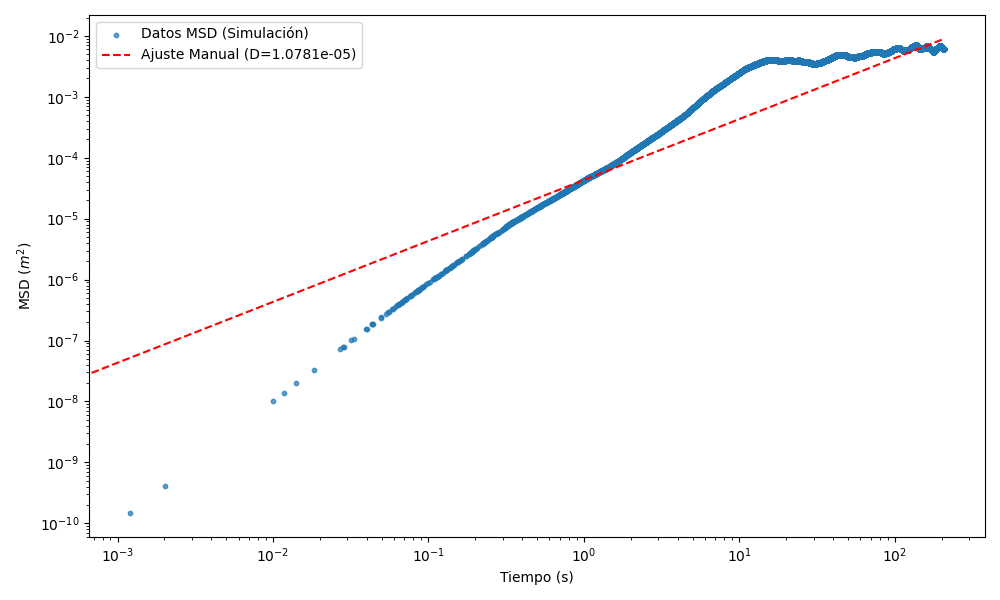
\includegraphics[width=1.10\linewidth]{photoMaterial/MSD_09.png}
    \end{column}
  \end{columns}
\end{frame}

\begin{frame}{Coeficiente de difusión}
  \begin{columns}
    \begin{column}{0.30\textwidth}
      \scriptsize \text{Input}
      \begin{itemize}
        \item L = \textit{0.03} m. 
        \item Velocidad inicial = \textit{0.01} m/s.
        \item Radio partículas = \textit{0.0015} m.
        \item Masa partículas = \textit{0.01} kg.
        \item Número de partículas = 250.
      \end{itemize}
    \end{column}
    \begin{column}{0.70\textwidth}
      %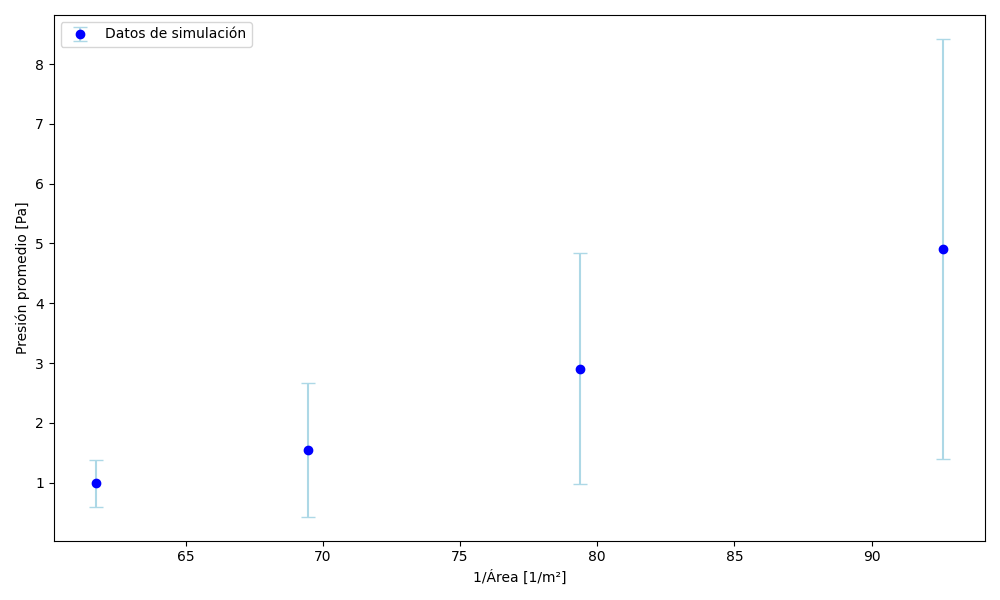
\includegraphics[width=0.75\linewidth]{photoMaterial/Presion_vs_area.png} ver si meterlo o no
      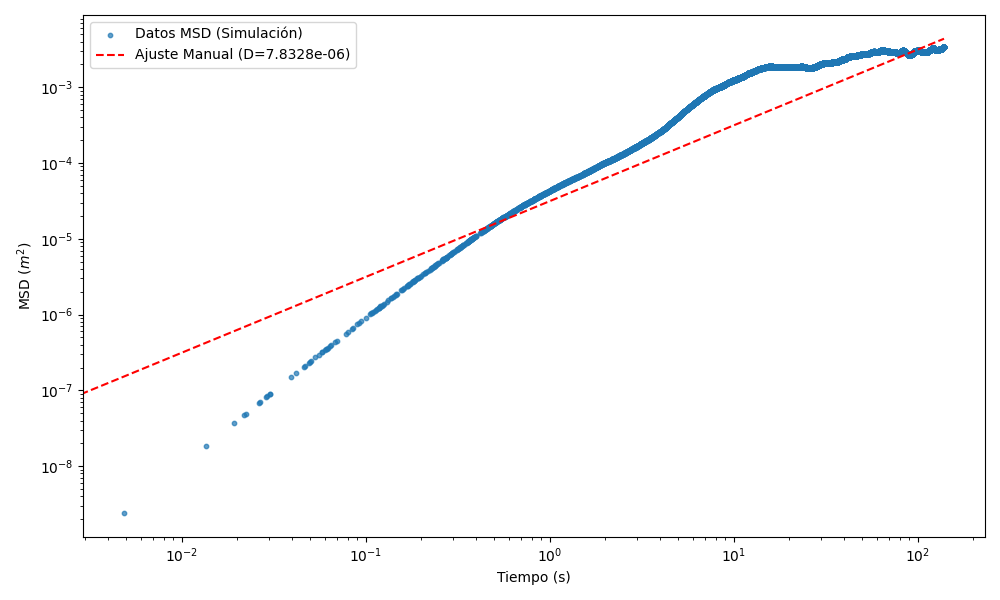
\includegraphics[width=1.10\linewidth]{photoMaterial/MSD_03.png}
    \end{column}
  \end{columns}
\end{frame}

% Conclusiones
\section{Conclusiones}
\begin{frame}{Conclusiones}
  \textbf{Primer estudio: Presión vs $A^{-1}$}
  \begin{itemize}
    \item Cuanta mayor area, menor es la presión.
    \item Luego de 10 segundos, todas las presiones entran en un régimen estacionario.
    \item NO se cumple la ley de los gases ideales ya que P no es cte.
  \end{itemize}
  \textbf{Segundo estudio: Coeficiente de difusión}
  \begin{itemize}
    \item Falta este análisis.
  \end{itemize}
\end{frame}

% Cierre
\begin{frame}{}
  \centering
  \Huge ¡Gracias por su atención!
\end{frame}

\end{document}

